\chapter{ Modelo Conceptual}


Um modelo conceptual consiste numa representação gráfica que permite visualizar as ligações entre diferentes conceitos e ideias. Este tipo de modelo é desenvolvido a partir da análise de uma base de dados, na qual a informação é organizada em entidades, atributos e chaves primárias, sendo também definidos os respetivos relacionamentos entre esses elementos. 
Numa fase inicial, é fundamental identificar as entidades a analisar, bem como os seus atributos, estabelecendo também as relações entre elas, de modo a representar de forma coerente a lógica do mundo real.

Na notação de Chen, as entidades são representadas por retângulos verdes, os atributos por elipses de cor roxa e as relações entre entidades por losangos amarelos inseridos em retângulos verdes. Os atributos-chave destacam-se por estarem sublinhados e a negrito.

Para definir corretamente as relações, a cardinalidade assume um papel essencial, pois indica quantas ocorrências de uma entidade podem estar associadas a outra. As relações podem ser classificadas em três tipos: um para um (1:1), um para muitos (1:N) e muitos para muitos (N:N). Este último ocorre quando uma entidade pode associar-se a várias ocorrências de outra entidade e vice-versa, originando normalmente uma entidade associativa.

Relativamente às ligações entre entidades, uma linha simples indica que a participação na relação é opcional, enquanto uma linha dupla representa uma participação obrigatória.
A fig. 1 apresenta um diagrama Entidade-Relacionamento (ER), criado com recurso ao \textit{software} TerraER.

\begin{figure}[h]
    \centering
    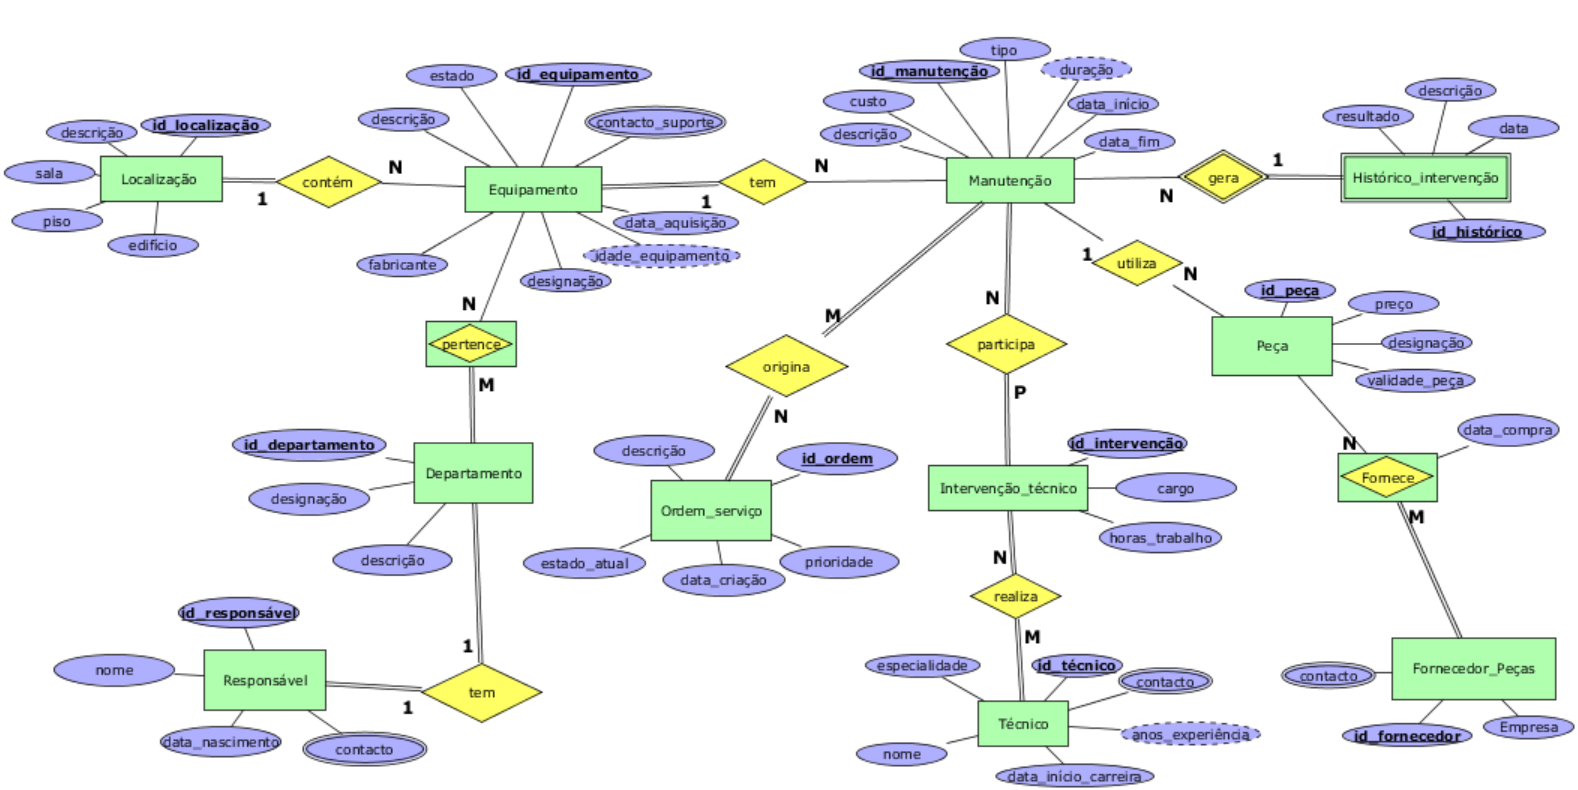
\includegraphics[width=1\textwidth]{./03-figuras/modelo_conceptual}
    \caption{Modelo Conceptual.}
\end{figure}


\section{ Entidades}
Entidades são objetos ou conceitos representados no banco de dados.  
Neste modelo, definiram-se as seguintes entidades:

\begin{itemize}
    \item \textbf{Localização}: Armazena informações sobre os locais onde os equipamentos se encontram;
    \item \textbf{Equipamento}: Contém os dados relativos aos equipamentos existentes;
    \item \textbf{Manutenção}: Regista informações sobre as manutenções realizadas nos equipamentos;
    \item \textbf{Histórico\_intervenção}: Guarda o histórico das intervenções efetuadas;
    \item \textbf{Peça}: Armazena dados sobre as peças utilizadas nas manutenções;
    \item \textbf{Fornecedor\_peças}: Contém informações sobre os fornecedores de peças;
    \item \textbf{Técnico}: Regista os dados dos técnicos responsáveis pelas intervenções;
    \item \textbf{Intervenção\_técnico}: Representa a participação dos técnicos nas intervenções;
    \item \textbf{Ordem\_serviço}: Guarda informações sobre as ordens de serviço criadas;
    \item \textbf{Departamento}: Contém os dados dos departamentos da organização;
    \item \textbf{Responsável}: Armazena informações sobre os responsáveis associados aos departamentos.
\end{itemize}


\section{ Atributos}
Atributos são características ou propriedades que descrevem uma entidade. Cada atributo tem
um tipo de dado associado, que define o tipo de valor que o atributo pode armazenar, como números
inteiros, texto, datas, entre outros.

De seguida, apresentam-se os atributos associados a cada uma das entidades.

\textbf{Localização:}
\begin{itemize}
    \item id\_localização - Identificador único da localização
    \item descrição - Descrição da localização
    \item sala - Sala onde se encontra o equipamento
    \item piso - Piso da localização
    \item edifício - Edifício correspondente
\end{itemize}

\textbf{Equipamento:}
\begin{itemize}
    \item id\_equipamento - Identificador único do equipamento
    \item descrição - Descrição do equipamento
    \item estado - Estado atual do equipamento
    \item fabricante - Fabricante do equipamento
    \item designação - Nome/designação do equipamento
    \item data\_aquisição - Data de aquisição do equipamento
    \item idade\_equipamento - Idade do equipamento
    \item contacto\_suporte - Contacto de suporte técnico
\end{itemize}

\textbf{Manutenção:}
\begin{itemize}
    \item id\_manutenção - Identificador único da manutenção
    \item tipo - Tipo de manutenção
    \item duração - Duração da manutenção
    \item data\_inicio - Data de início da manutenção
    \item data\_fim - Data de fim da manutenção
    \item custo - Custo da manutenção
    \item descrição - Descrição da manutenção
\end{itemize}

\textbf{Histórico\_Intervenção:}
\begin{itemize}
    \item id\_histórico - Identificador único do histórico
    \item descrição - Descrição da intervenção
    \item resultado - Resultado da intervenção
    \item data - Data da intervenção
\end{itemize}

\textbf{Peça:}
\begin{itemize}
    \item id\_peça - Identificador único da peça
    \item designação - Nome/designação da peça
    \item preço - Preço da peça
    \item validade\_peça - Validade da peça
\end{itemize}

\textbf{Fornecedor\_peças:}
\begin{itemize}
    \item id\_fornecedor - Identificador único do fornecedor
    \item empresa - Nome da empresa fornecedora
    \item contacto - Contacto do fornecedor
\end{itemize}

\textbf{Técnico:}
\begin{itemize}
    \item id\_técnico - Identificador único do técnico
    \item nome - Nome do técnico
    \item especialidade - Especialidade do técnico
    \item contacto - Contacto do técnico
    \item anos\_experiência - Anos de experiência
    \item data\_inicio\_carreira - Data de início de carreira
\end{itemize}

\textbf{Intervenção\_técnico:}
\begin{itemize}
    \item id\_intervenção - Identificador único da intervenção
    \item cargo - Função do técnico na intervenção
    \item horas\_trabalho - Número de horas trabalhadas
\end{itemize}

\textbf{Ordem\_serviço:}
\begin{itemize}
    \item id\_ordem - Identificador único da ordem de serviço
    \item descrição - Descrição da ordem
    \item estado\_atual - Estado atual da ordem
    \item data\_criação - Data de criação da ordem
    \item prioridade - Prioridade da ordem
\end{itemize}

\textbf{Departamento:}
\begin{itemize}
    \item id\_departamento - Identificador único do departamento
    \item designação - Nome/designação do departamento
    \item descrição - Descrição do departamento
\end{itemize}

\textbf{Responsável:}
\begin{itemize}
    \item id\_responsável - Identificador único do responsável
    \item nome - Nome do responsável
    \item data\_nascimento - Data de nascimento
    \item contacto - Contacto do responsável
\end{itemize}